% diagrams/english/arbol-navidad.tex -- el árbol de Navidad, para "Read
% and colour": el árbol en tres pisos, la estrella de arriba, las bolas,
% el tronco en su maceta y un regalo debajo.
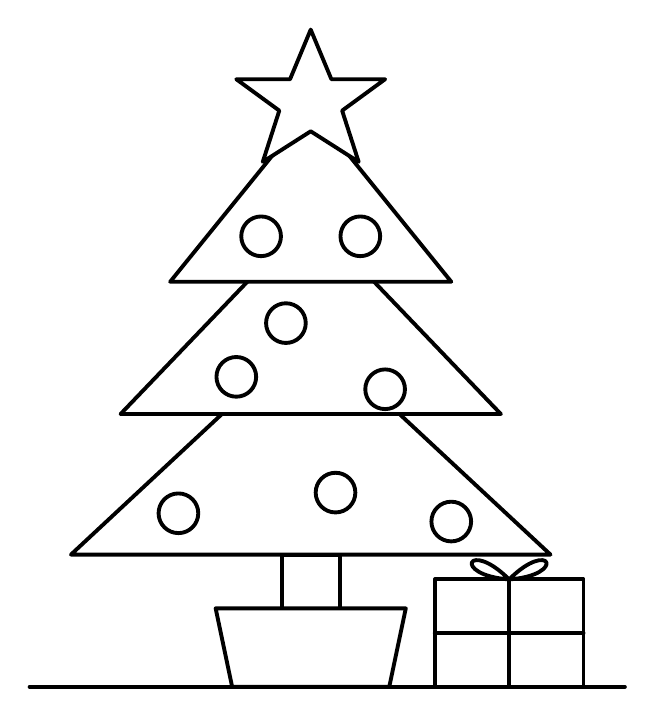
\begin{tikzpicture}[line width=1.4pt, line cap=round, line join=round, scale=1.05]
  % el tronco y la maceta
  \filldraw[fill=white] (-0.35,0.9) rectangle (0.35,1.6);
  \filldraw[fill=white] (-0.95,0) -- (-1.15,0.95) -- (1.15,0.95) -- (0.95,0) -- cycle;
  % los tres pisos del árbol, de abajo arriba
  \filldraw[fill=white] (-2.9,1.6) -- (2.9,1.6) -- (0,4.3) -- cycle;
  \filldraw[fill=white] (-2.3,3.3) -- (2.3,3.3) -- (0,5.7) -- cycle;
  \filldraw[fill=white] (-1.7,4.9) -- (1.7,4.9) -- (0,7.0) -- cycle;
  % la estrella
  \filldraw[fill=white] (0,7.95) -- (0.25,7.35) -- (0.9,7.35) -- (0.38,6.97) -- (0.58,6.35)
    -- (0,6.72) -- (-0.58,6.35) -- (-0.38,6.97) -- (-0.9,7.35) -- (-0.25,7.35) -- cycle;
  % las bolas
  \foreach \p in {(-1.6,2.1), (0.3,2.35), (1.7,2.0), (-0.9,3.75), (0.9,3.6), (-0.3,4.4),
                  (-0.6,5.45), (0.6,5.45)} {
    \filldraw[fill=white] \p circle (0.24);
  }
  % el regalo, al lado del tronco
  \filldraw[fill=white] (1.5,0) rectangle (3.3,1.3);
  \draw (2.4,0) -- (2.4,1.3); \draw (1.5,0.65) -- (3.3,0.65);
  \draw (2.4,1.3) .. controls (1.9,1.8) and (1.7,1.35) .. (2.4,1.3)
        .. controls (3.1,1.35) and (2.9,1.8) .. (2.4,1.3);
  % el suelo
  \draw (-3.4,0) -- (3.8,0);
\end{tikzpicture}
